% !Mode:: "TeX:UTF-8" 

\BiChapter{基于注意力机制的卷积神经网络社交媒体文本立场分析}{Methods of inserting figures}

\BiSection{引言}{Figures inserting standard from graduate school}
近年来,深度学习的研究越来越深入,在各个领域也都获得了不少突破性的进展。基于注意力(attention)机制的神经网络成为了最近神经网络研究的一个热点,引起了研究者的广泛关注。在神经网络实现预测任务时,引入注意力机制能使训练重点集中在输入数据的相关部分,而不是无关部分。在社交媒体文本立场分析任务中, 不管是基于传统特征工程的机器学习模型SVM和基于端到端的深度学习的RNNs,CNNs等神经网络模型,都忽略主题目标信息对社交媒体立场分析的重要作用,这样建立模型存在的不合理性,为了更好的引入主题目标信息帮助提高社交媒体文本立场分析任务的性能,在本章引入基于注意力机制的神经网络模型。通过不同的权重,注意力机制能根据主题目标更好的对微博或者文本信息进行不同重要性的关注,使模型更加聚焦在对主题目标立场分析重要的信息上。实验结果表明,基于注意力机制的神经网络模型在社交媒体文本立场分析任务中取得了相当不错的效果,证明了注意力机制的有效性。

本章 4.2 节首先介绍深层记忆网络的重要机制及架构, 4.3 节介绍深层记忆网络在社交媒体文本立场分析中的应用,4.4 节介绍实验设置和结果的分析,4.5 节作出本章小结。

\BiSection{注意力机制的卷积神经网络模型的社交媒体文本立场分析}{Captions and descriptions of figures}

近年来,基于深度学习已经在图像识别、语音识别和自然语音处理上上获得了重要的进展。在自然语言处理任务中,注意力机制在神经网络机器翻译、序列标注、层次性文本分类上取得突破性提高。注意力机制将对信息呈现不同的关注程度,通过聚焦在重要的信息上,达到模型性能的特点。本节!!!!!!
\BiSubsection{注意力机制}{}
注意力机制最早应用在图像识别领域上,研究人员研究的动机其实也是受到人类注意力机制的启发。人们在进行观察图像的时候,并不是一次就把整幅图像的每个位置像素都看过,大多是根据需求将注意力集中到图像的特定部分。而且人类会根据之前观察的图像学习到未来要观察图像注意力应该集中的位置。

注意力机制除在图像识别和语音识别上取得巨大的成功,近期在基于RNNs的端到端的编码解码的机器翻译、序列标注和层次文本分类等任务取得突破。在自然语言处理任务中,首先引入注意力机制的是神经网络机器翻译。神经网络机器翻译其实就是一个典型的序列到序列模型,也就是一个编码解码模型。由于基于注意力机制的卷积神经网络模型的注意力机制很类似于机器翻译中的注意力机制,这里将简单介绍下机器翻译中的编码解码注意力机制模型。
\begin{figure}[htbp]
	\centering
	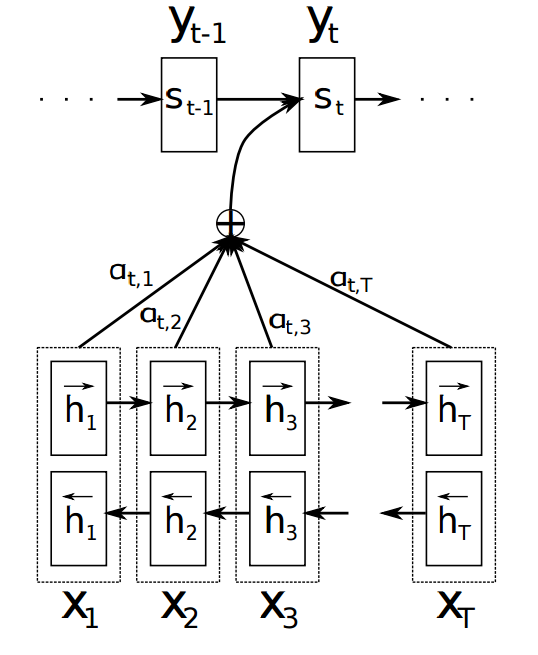
\includegraphics[width = 0.4\textwidth]{NMT.png}
	\caption[rnn_vanish]{注意力机制神经翻译模型}
\end{figure}

传统的神经翻译模型编码阶段里面用的是RNNs模型,这样每个单词的表达不仅能包含前一个单词的信息,还可以包含后一个; RNNs按输入序列的顺序,生成同样顺序的隐藏层状态,这样它就既包含当前单词的前一个单词信息,也包含后一个信息; 这个状态之后将被用于解码阶段部分。
\begin{equation}\label{lstm_f} h_t = f(x_t,h_{t-1}) \end{equation}

其中编码信息为
\begin{equation}\label{lstm_f} c = q(\lbrace h_1,...h_{T_x} \rbrace ) \end{equation}

其中$h_t$是时间$t$的隐藏状态,$c$向量是从序列信息得到的压缩向量,通常$f$和$q$是非线性函数,例如SutSkever[XXX]等用的是LSTM作为$f$函数,把前向循环网络的最后一个隐状态当做最好的压缩向量,$q(\lbrace h_1,...h_{Tx} \rbrace )=h_T$

在解码阶段,解码器的作用是根据编码的信息和已经输出的信息来预测下一个词最有可能的单词,可以用下面公式~\ref{rnndecoder}~表示
\begin{equation}\label{rnndecoder} p(y) = \prod_{t=1}^{T} p(y_t|\lbrace y1,...,y_{t-1} \rbrace , c) \end{equation}
当$y=(y1,...,y_{T})$,若用RNN式的结构,每个的条件概率如公式\ref{rnndecodery}
\begin{equation}\label{rnndecodery} p(y_t|\lbrace y1,...,y_{t-1} \rbrace , c) = g(y_{t-1},s_t, c)\end{equation}

而基于注意力机制的神经翻译模型的条件概率公式如下
\begin{equation}\label{} p(y_t|\lbrace y1,...,y_{t-1},x \rbrace , c) = g(y_{t-1},s_t, c_i)\end{equation}
其中$s_i$是RNN的隐状态,其中的计算公式如下
\begin{equation}\label{} s_i = f(s_{i-1},y_{i-1}, c_i)\end{equation}
其中从传统的神经翻译模型做出的改进是对于每一个不同的输出,它所依据的上下文压缩向量$c_i$不在是同一个压缩向量$c$,$c_i$的计算是通过$(h_1,...,h_{T_x})$的加权所得。$h_i$虽然包含所以所有的输入信息,但是主要存储了$x_i$的信息。其中$c_i$的计算公式如\ref{c1}所示
\begin{equation}\label{c1} c_i = \sum_{j=1}^{T_x} \alpha_{ij}h_i\end{equation}
其中注意力变量$\alpha{ij}$的计算公式如下
\begin{equation}\label{alpha} \alpha_{ij} = \frac{exp(e_{ij})}{\sum_{k=1}^{T_x}exp(e_{ik})}\end{equation}
其中$e_{ij}$的计算公式如下
\begin{equation}\label{eij} \alpha_{ij} = a(s_{i-1},h_j)\end{equation}

注意力机制的加入使得神经网络翻译模型具有更强的对句子翻译建模能力,使模型在翻译当前词语时关注和词语的更相关的内容,忽略不相关的内容。通过可视化注意力$\alpha{ij}$可显示看出在翻译不同词语时,对原语言关注的内容是不一样的,例如在中文翻译中的注意力矩阵如下图\ref{english2china}所示
\begin{figure}[htbp]
	\centering
	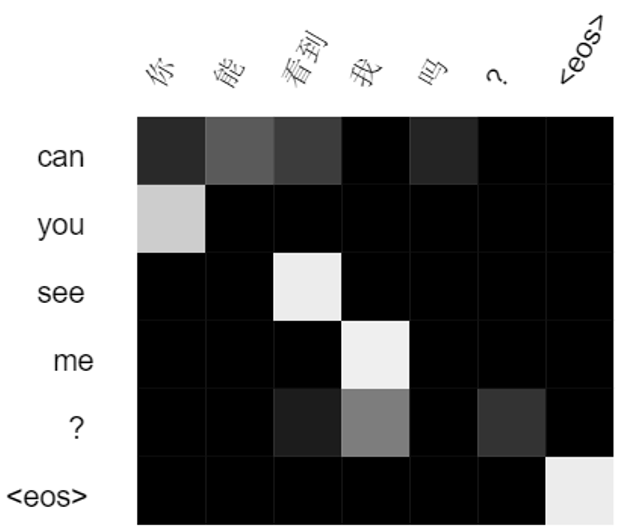
\includegraphics[width = 0.5\textwidth]{mnt_visual.jpg}
	\caption[english2china1]{中英文翻译注意力矩阵}
	\label{english2china}
\end{figure}

\BiSubsection{卷积神经网络}{xxl}

卷积原是常用在积分变换等领域的数学概念。现在被广泛应用于计算机视觉、自然语言处理和语音识别等任务中。卷积神经网络是对神经网络模型的改进。卷积层把原来的全连接改成局部连接权值共享,既可以大大缩减参数个数,又可以适应不同区域统计特性一样的特征。下采样层可以利用局部信息采样特征图得到更低纬度的特征,提高模型的泛化能力,防止训练的分类器过拟合。

根据不同任务,卷积神经网络的输入矩阵处理方式也不全相同。用于图片分类时,输入矩阵为像素点矩阵,用于文本分类时,输入矩阵为相同维度的词向量以一行一个词拼接。卷积神经网络使用预设石村的卷积核作为过滤器,与输入矩阵做卷积操作。

以文本卷积神经网络为例,当输入矩阵的词向量维数为$d$,句子长度为$l$,输入矩阵的大小为$A\in R^{l\times d}$, $A[i:j]$表示输入矩阵中从第$i$行到第$j$行的子矩阵。尺寸为$h$的过滤器对矩阵$A$做卷积操作,输出矩阵$O\in R^{s-h+1}$如公式~\ref{conv1}~所示,
\begin{equation}\label{conv1}
O_i=W\cdot A[i:i+h-1]
\end{equation}
其中,$i$为从1到$s-h+1$的数列。

将输出矩阵与偏置$b$相加,放入激活函数中处理,即可得到卷积层的输出$C_i$。

卷积层一般会连接下采样层。在自然语言处理任务重,下采样层通常使用KMAX池化函数,所以下采样层也被称为池化层。池化层既可以对卷积层的输出再次降维从而组合更大窗口范围的特征,同时也可以将不同尺寸的卷积核得到的特征构建为固定长度的输出,避免了不同输入矩阵大小表示的差异。之后的向量通常会连接Dropout层,随机抛弃一些节点,也是为了减少过拟合现象同时可以增强网络的训练效果。最后的全连接分类层通常使用softmax函数,基于多卷积核文本的CNN分类框架图如~\ref{multiCNN}~所示

\begin{figure}[htbp]
	\centering
	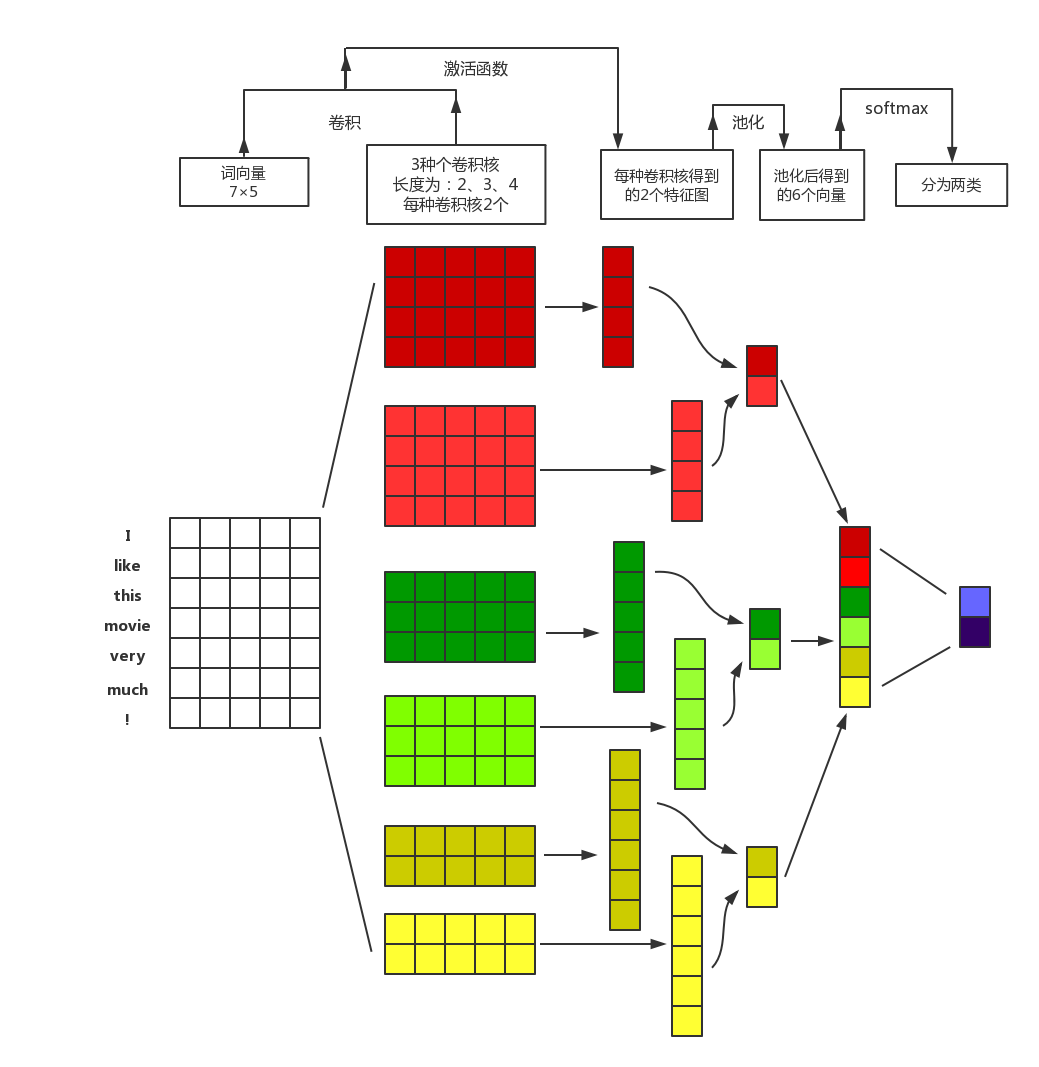
\includegraphics[width = 0.95\textwidth]{text_cnn.png}
	\caption{多卷积核文本CNN}
	\label{multiCNN}
\end{figure}

\BiSubsection{注意力机制卷积神经网络社交媒体文本立场分析}{}
基于注意力机制在神经网络翻译模型、序列标注、层次文本分类等领域取得的成功。文本多卷积核CNN模型在文本分类上的也取得了较好的效果。在社交媒体的文本立场分析上,由于当前研究没有一种有效把主题目标信息以合适的方式结合在文本的立场分析中,但是主题目标对文本立场分析又有着举足轻重的影响。为了主题目标信息没有合适引入的缺点,本文提出一种以注意力机制引入主题目标信息,在注意力的基础上,用多卷积核文本CNN模型提取文本立场的模型,本节结合立场分析数据集中的中文实例数据,描述注意力机制卷积神经网络在该问题中的主要工作流程和重要计算方法。
\begin{figure}[htbp]
	\centering
	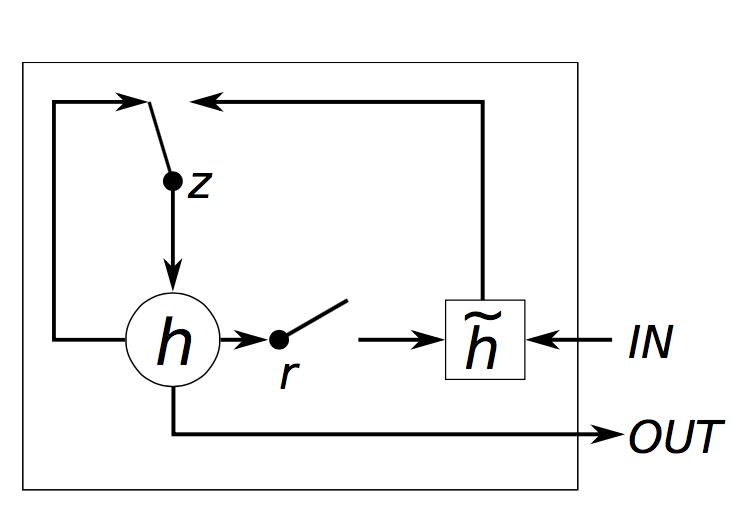
\includegraphics[width = 0.6\textwidth]{gru.png}
	\caption[rnn_vanish]{GRU内部结构}
	\label{gru}
\end{figure}
文本引入了双向GRU(Gated recurrent unit)用来编码文本信息,相对于RNN单元,GRU也能够缓解递归神经网络的梯度消失的问题,相对于LSTM单元,GRU具有更少的参数和更快的运算速度,因此本文利用例如GRU编码信息。相对于LSTM单元有输入门、遗忘门和输出门的三个门单元,按图~\ref{gru}~所示,GRU采取了一种更加简洁的建模方式,只需要保持更新门和重置门,更新门表示隐藏单元有多少信息需要保留下来,重置门表示都是隐藏单元信息参与输入的更新,同时也删除了LSTM的记忆单元,具体的门的更新和输出更新公式如下

\begin{equation}\label{conv1} z_t=\alpha_g(W_zx_t+U_zh_{t-1}+b_z) \end{equation}
\begin{equation}\label{conv1} r_t=\alpha_g(W_rx_t+U_rh_{t-1}+b_r) \end{equation}
\begin{equation}\label{conv1} h_t=z_t\odot h_{t-1} + (1-z_t)\odot \alpha(W_hx_t+U_h(r_t\odot h_{t-1})+b_h) \end{equation}



本节以“深圳禁摩限电”为话题目标,微博文本“支持深圳交警。电单车继续治理”为例,按本节模型的5个层次,描述注意力机制卷积神经网络的立场分析的过程,具体模型的结构如图~\ref{GRU_CNN}~所示

\begin{figure}[htbp]
	\centering
	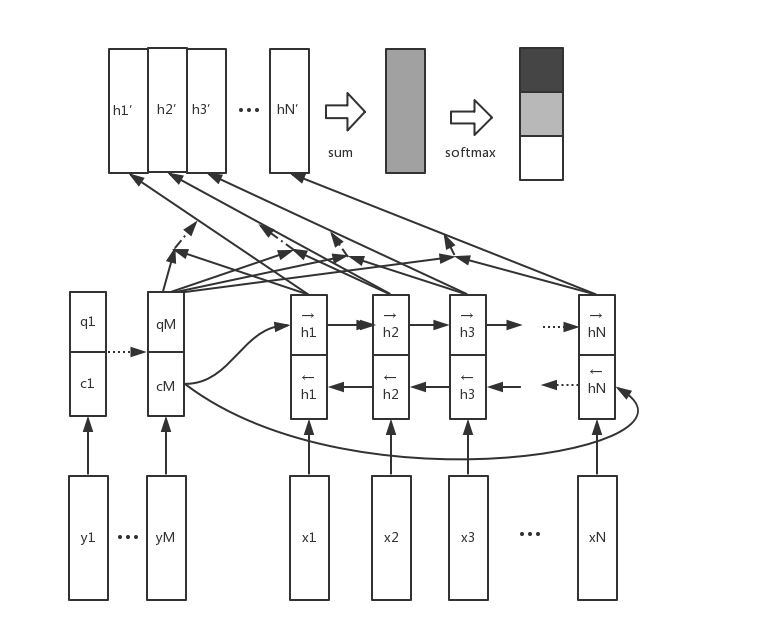
\includegraphics[width = 0.61\textwidth]{a_bi_gru_cnn.png}
	\caption[]{条件编码长短期记忆}
	\label{GRU_CNN}
\end{figure}

(1) 输入层

先将话题目标和微博文本经过预处理操作,然后通过分词工具把话题目标和微博文本进行划分,对于同一个话题目标,微博文本分词后句子长度有可能不一致,为了方便后续神经网络框架中的批量的并行计算,英文语料统计选择30为固定长度,中文语料统计后截取50为固定长度,长度超过固定长度进行截断操作,不够的进行补齐词表中规定 <PAD> 关键词。如上述微博文本最后转换成”支持深圳交警。电单车继续治理 <PAD> ... <PAD>“,而话题目标也需要进行分词操作,例如例子中“深圳禁摩限电”根据结巴分词分割成“深圳”、“禁摩”和“限电”三个词组。经过此层后主题目标信息和微博文本信息可以转换成以下形式,m,n分布为主题目标和微博文本的长度。
\begin{equation}\label{target_info} Target= \lbrace w_1,w_2...w_m\rbrace \end{equation}
\begin{equation}\label{text_info} Text=\lbrace w'_1,w'_2...w'_n\rbrace  \end{equation}

(2)词向量嵌入层

词向量的嵌入层,此层的功能是对输入的每一次词检索其词向量 (lookup操作),后续实验词向量的预训练由 GloVe 模型在大量无监督语料上训练可得,预训练的词向量维度为200,且把词向量设置为可训练,随神经网络模型的训练动态调整权重。经过此层后主题目标信息和微博文本信息可以转换成以下形式。
\begin{equation}\label{target_info} Target_v= \lbrace y_1,y_2...y_m\rbrace \end{equation}
\begin{equation}\label{text_info} Text_v=\lbrace x_1,x_2...x_n\rbrace \end{equation}

(3)主题目标编码与文本编码层

由于微博和Twitter文本立场分析中的主题目标包含的词语相对较少,为了减少模型的参数空间,因此编码主题目标信息的方法是平均所有词向量。微博或Twiiter文本包含了文本立场分析的绝大部分信息,双向的GRU单元能比单向更好抽取文本中的信息,对于当前词的隐藏状态包含前向和后向的GRU隐状态。具体的转换如公式所示。
\begin{equation}\label{target_info} q=\frac{\sum_{m}^{i=1}y_i}{m} \end{equation}
\begin{equation}\label{target_info} h^→_i = GRU^→(h^→_{i-1}, x_i) \end{equation}
\begin{equation}\label{text_info}  h^←_i = GRU^→(h^←_{i+1}, x_i) \end{equation}
\begin{equation}\label{text_info}  h_i = [h^→_{i-1}, h^←_{i+1}] \end{equation}

(4)注意力机制计算与基于注意力的隐藏状态合成

通过结合主题目标编码信息$q$和微博的文本信息的基于双向GRU模型的隐状态$h_i$,分布计算主题目标对每个词的关注程度,对于文本分析影响大的词,注意力机制会给予大的权重,反过来对于无用信息,注意力机制则会给予小的权重。分别计算每个词的权重后,原隐状态点城注意力的权重形成基于注意力的隐藏状态,具体的计算公式如下
\begin{equation}\label{conv1} e_i=att(h_i,q)=W^t_n(tanh(W_{ah}h_i+W_{aq}q+b_a))+b_m \end{equation}
\begin{equation}\label{conv1} a_i=\frac{exp(e_i)}{\sum_{N}^{n=1}exp(e_n)} \end{equation}
\begin{equation}\label{conv1} h'_i=a_i \odot h_i \end{equation}

(5)多窗口核卷积与池化操作

模型初始化不同大小的过滤器窗口,每种尺寸的窗口随机初始化若干参数。图中所示窗口大小w为2,并随机初始化多个不同的过滤器。所得向量将送入修正线性单元(Rectified Linear Units,ReLU)等非线性目标激活函数中,池化操作将卷积层中每个卷积过滤器所得长度为N-h+1的向量使用最大池化操作(max pooling),池化操作能减低参数维度,减少计算复杂度。具体公式如下
\begin{equation}\label{conv1} c_i=W*h[i:i+w-1]+b \end{equation}
\begin{equation}\label{conv1} c=Max(c_1,c_2,...,c_n) \end{equation}

(6)全连接分类层
把每个卷积核经过池化操作的值拼接在一起作为模型最后的特征向量,对特征向量连接一个以三个输出单元的全连接层。全连接层输出外接Softmax归一化函数,输出的值为归一化到0-1之间的实数值,代表的意义为模型分类到某一个立场的概率,具体公式如下。
\begin{equation}\label{conv1} ouput_i=Softmax(W_{h3}C+b_{h3}) \end{equation}



\BiSection{实验设置及结果分析}{hello}

本节主要介绍基于注意力机制的卷积神经网络模在NLPCC2016中文微博数据集和SemEval2016英文Twitter数据集中的实验设置及结果分析。通过对样例的可视化注意力机制分析模型是否能抓取对主题目标其关键性作用的信息,解释模型能提高文本立场分析的性能的原因。本节包含两部分: 4.4.1小节简介有关实验的数据集、评价方法、数据预处理词和词向量的训练。4.4.2 小结介绍模型在两个数据集上的结果、对样例的注意力机制可视化结果分析和对比其他模型的结果与分析。


\BiSubsection{实验设置}{}

本章通过在中英文社交媒体数据集上的实验,验证基于注意力机制的卷积神经模型在文本立场分析任务上的有效性。数据集包含NLPCC2016中文微博立场分析数据集和SemEval2016英文Twitter立场分析数据集。由于本章实验使用与第三章实验一样的数据集,这里将不再赘述数据集的相关分布,有关数据集的详细分布参考第三章实验章节有关数据集的介绍,训练集、验证集与测试集的划分也与第三章相同。

有关评价方法也与第三章相同,对于同一个数据集内所以主题目标,分别计算其“支持”立场和“反对”立场的F1值,取其两者的平均值作为每个主题的平均F1值。模型在一个数据集上的总体性能通过无差别对待每一个主题目标计算总的“支持”立场与“反对”立场的F1值,两者F1值的平均数作为整个数据集的微平均F1值,微平均F1值代表了模型在数据集上的总体性能,其作为模型最重要的评价指标。有关F1值与微平均F1值的具体计算公式参考第三章的相关介绍。

中英文本数据的预处理步骤主要步骤有转换大小写、过滤停用词与对低频词用“UNKONW”关键词替代。中文本分词工具为结巴分词,英文Twiiter的分词为CMU专门为Twiiter文本定制的Twitter NLP tool中的分词器。对于英文固定的文本长度为30个词,中文微博为固定60个词。

英文语料的词向量训练通过GloVe算法在20亿Twitter文本语料训练而成,其中包含了120万个词,词向量维度为100。中文微博语料是通过Word2Vec算法在大量微博语料中训练所得,其中包含了17万个词,词向量的维度也为200。


\BiSubsection{实验结果及分析}{}
本文针对中英文数据集内容相差较大的特点,给两个不同的数据集设置不同的超参数,使模型在两个数据集上均取得较好的性能。取出训练集合的10\%作为验证集参与模型的选择。本章提出的基于注意力机制的卷积神经网络的核心超参数主要集中在通过Bi-GRU模块进行注意力矩阵和隐藏层的产生的循环神经网络的模块,最后在注意力矩阵作用下的隐藏层提取特征的卷积神经网络模块。处理英文数据的双向GRU的隐藏层的单元数为64,处理中文数据的双向GRU的隐藏层单元数为100。处理英文卷积神经网络的词窗口大小为2,3,4,每个词窗口有50个卷积核,处理中文卷积神经网络的词窗口大小为3,4,5。每一个词窗口有50个卷积核。对词向量抽取层的dropout概率为0.2,对GRU内部记忆单元的dropout概率为0.3,批处理单元样本个数为16。对训练参数的L2正则项为1e-6。选取0.001的学习率的Adam优化方法。模型训练100轮,保留在验证集合性能最好的模型参数。

\begin{table}[htbp]
	\caption[param]{基于注意力机制的卷积神经网络模型超参数集}
	\label{param}
	\vspace{0.5em}\centering\wuhao
	\begin{tabular}{ccc}
		\toprule[1.5pt]
		序号& 超参数名称 &数值\\
		\midrule[1pt]
		0 &词向量大小& 英文 100, 中文 200\\
		1 &GRU隐藏层单元& 英文 64,中文 100\\
		2 &卷积窗口大小&英文[3,4,5],中文[2,3,4]\\
		3 &卷积核数目& 50\\
		4 &Embedding层dropout& 0.2\\
		5 &GRU内部drought& 0.3\\
		6 &批处理大小& 32\\
		7 &L2 正则化参数 &1e-6\\
		8 &全量迭代次数& 50\\
		9 &梯度优化方法& Adam\\
		10 &学习率& 0.001\\
		\bottomrule[1.5pt]
	\end{tabular}
\end{table}

使用上述超参数训练模型,基于注意力机制的卷积神经网络模型在SemEval2016数据集上的表现表~\ref{a_bi_gru_cnn_semeval}~所示。
\begin{table}[htbp]
	\caption[table123]{基于注意力机制的卷积神经网络模型在各个话题试验性能(SemEval数据集)}
	\label{a_bi_gru_cnn_semeval}
	\vspace{0.5em}\centering\wuhao
	\begin{tabular}{cccccccc}
		\toprule[1.5pt]
		主题目标& $P_{favor}$&$R_{favor}$&$F_{favor}$&$P_{against}$&$R_{against}$&$F_{against}$&$F_{average}$ \\
		\midrule[1pt]
		Atheism&0.5455&0.3750&0.4444&0.8645&0.8375&0.8508&0.6476\\
		Climate Change&0.7532&0.9675&0.8470&0.0000&0.0000&0.0000&0.4235\\
		Feminist Movement&0.3333&0.4483&0.3824&0.7843&0.6557&0.7143&0.5483\\
		Hillary Clinton&0.4423&0.5111&0.4742&0.6733&0.7907&0.7273&0.6007\\
		Legal. of Abortion&0.4773&0.4565&0.4667&0.7791&0.6720&0.7216&0.5941\\
		合并统计&0.5678&0.6612&0.6145&0.7682&0.7231&0.7456&0.6801\\
		\bottomrule[1.5pt]
	\end{tabular}
\end{table}

如表~\ref{a_bi_gru_cnn_semeval}~所示,以下分析模型的结果。基于注意力机制的卷积神经网络模型在所有主题目标下微平均F1值的指标为0.6701,其在所有主题目标“支持”立场的F1值为0.5145,而“反对”立场的总体F1值有0.7456。由于原始数据的分布,模型在“反对”立场的性能还是优于“支持”立场,原英文数据集的分布如表~\ref{englishdata}~所示。模型对各个主题目标的性能有较大的差异,在“Athesim”主题目标下性能能达到0.647,而在主题目标“Climate Change is a Real Concern”中,由于训练集中“支持”立场是“反对”立场的10多倍,模型还是没有克服这个数据分布的缺陷,没有将任意一个样本的归类为“反对”。

\begin{table}[htbp]
	\caption[table123]{基于注意力机制的卷积神经网络模型在各个话题试验性能(NLPCC数据集)}
	\label{chinese_a_bi_gru_cnn_semeval}
	\vspace{0.5em}\centering\wuhao
	\begin{tabular}{cccccccc}
		\toprule[1.5pt]
		主题目标& $P_{favor}$&$R_{favor}$&$F_{favor}$&$P_{against}$&$R_{against}$&$F_{against}$&$F_{average}$ \\
		\midrule[1pt]
		iPhone SE&0.6333&0.5067&0.5630&0.7262&0.5865&0.6489&0.6059\\
		春节放鞭炮&0.7100&0.8068&0.7553&0.7826&0.7660&0.7742&0.7648\\
		俄在叙反恐行动&0.6389&0.4894&0.5542&0.5463&0.6860&0.6082&0.5812\\
		开放二胎政策&0.7961&0.8283&0.8119&0.8765&0.7474&0.8068&0.8093\\
		深圳禁摩限电&0.6353&0.8571&0.7297&0.8667&0.8273&0.8465&0.7881\\
		总计&0.6929&0.6945&0.6937&0.7532&0.7239&0.7386&0.7161\\
		\bottomrule[1.5pt]
	\end{tabular}
\end{table}

在NLPCC2016数据集上,各主题目标的性能如表~\ref{chinese_a_bi_gru_cnn_semeval}~所示。基于注意力机制的卷积神经网络模型在所有主题目标下微平均F1值的指标为0.7161,其在所有主题目标“支持”立场的F1值为0.6937,而“反对”立场的总体F1值有0.73856,“支持”立场与“反对”立场在整体的F1值较为相近,因此模型在此数据集上的性能也比英文数据要高0.034左右。由于NLPCC2016中文数据集在各主题目标下立场类标分布相对较平均,没有出现类似与英文数据集中“Climate Change is a Real Concern”单个主题目标平均F1值只有0.4的现象,但是模型在各个不同主题目标下的性能还是有较大的差距,模型在”开放儿童政策“的主题目标下平均F1值达到了0.8093,但是在“俄在叙反恐行动”主题目标下的平均F1值只有0.581,体现了不同主题目标下,立场分析难易程度也相差较大。


上述实验论证和合适的方式引入主题目标信息可以提升文本立场分析的性能,为了验证提出的条件编码LSTM模型的有效性和不足,以下通过实验结果对比其他研究人员在文本研究中模型。由于两个数据集来源于不同的评测任务,因此分别从SemEval2016英文数据集和NLPCC2016中文数据集挑选出较好系统和本章提出的条件编码LSTM进行比较。

在SemEval数据集合上,引入以下模型是作为对比模型

(1)MITRE, SemEval2016 Twitter立场分析评测任务第一名,收集大量的无标注数据。通过分析筛选出多个\#话题标签,建立LSTM模型去预测文本的标签。先训练预测标签的模型,而后在预训练好的模型上做立场分析的任务上的微调,此模型基于大量无标注样本的迁移学习,需要大量无标注任务和手工筛选特别话题标签。

(2)TakeLab   SemEval2016 Twitter立场分析评测参赛模型,融合了随机森林,逻辑回归,支持向量机等多种机器学习的集成学习方法,各模型利用大量人工构造的特征。

(3)ECNU  SemEval2016 Twitter立场分析评测华东师范大学参赛模型,采用了传统语义特征、主题目标特征、相似性特征、情感字典特征、主题模型特征和词向量特征的特征工程的传统机器学习方法

(4) BiText-On-Target本章出的基于主题目标的条件的双向LSTM文本编码模型

四个模型在SemeEval2016的各主题目标下单个平均F1值如图~\ref{chart_semeval_best_model}~所示
\begin{figure}[htbp]
	\centering
	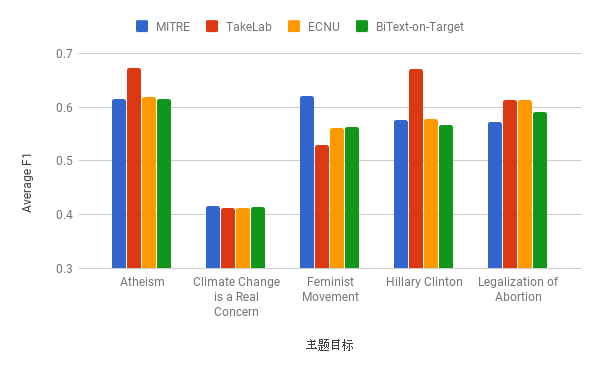
\includegraphics[width = 1.0\textwidth]{chart_semeval_best_model.png}
	\caption[rnn_vanish]{模型在SemeEval2016各主题目标平均F1值分布}
	\label{chart_semeval_best_model}
\end{figure}
所以模型在”Climate Change is a Real Concern“主题目标上的性能都较差,没有一个模型的性能超过了0.43的平均F1值。数据类标分布极度不平均,训练集与测试集分布差异大的问题的问题影响了所有模型,4个模型都没克服这个缺陷。基于特征工程的TakeLab和ECNU模型对”Legal of Abortion“主题目标的性能相对较好,基于深度学习的MITRE模型和BiText-On-Target模型相对较差,在此主题目标下,基于统计的特征具有更好的立场分析区分度。TakeLab在”Atheism“和”Hillary Clinton“主题目标的效果远高于其他模型,原因是其运用了集成随机森林,逻辑回归,支持向量机等多种分类器,模型相对强健。BiText-On-Target模型在所有的主题目标下都拥有相对稳定的效果,虽然没在任意主题目标取得最好的立场分析效果,但所有主题目标的效果都不是很差,相对于其他三个模型更加稳定和强健。

上述模型在SemEval数据集下的综合”支持“和”反对“的F1值和总体微平均F1值的性能如下表~\ref{semeval_res}~所示

评测最好的模型MITRE的的微平均F1值为0.678,本章提出的模型BiText-On-Target取得了0.671的平均F1值,此模型在评测中取得3(20)的成绩。虽然模型的性能比MITRE的相比低了0.007,但MITRE需要大量的无标注数据,TakeLab模型虽然在某些主题目标下取得较好的F1平均值,但是对于总体的”支持“和“反对”立场微平均F1值的效果不如BiText-On-Target模型。

\begin{table}[htbp]
	\caption[table123]{各模型在立场分析测试集中的性能表现(SemEval 数据集)}
	\vspace{0.5em}\centering\wuhao
	\label{semeval_res}
	\begin{tabular}{cccccccc}
		\toprule[1.5pt]
		主题目标& $F_{favor}$&$F_{against}$&$F_{average}$ \\
		\midrule[1pt]
		MITRE&0.5932&0.7633&0.6782\\
		TakeLab&0.6093&0.7273&0.6683\\
		ECNU&0.6055&0.7054&0.6555\\
		BiText-On-Target&0.6112&0.7314&0.6713\\
		\bottomrule[1.5pt]
	\end{tabular}
\end{table}

上述统计说明模型在SemEval英文数据的性能,以下将在NLPCC2016中文数据集对比评测中的模型,对比的模型如下所示
(1)RUC-MMC NLPCC2016 立场分析评测任务第一名,提取同义词,TF-IDF,n-gram等作为特征结合支持向量机和随机森林分类器
(2)Top-Team NLPCC2016立场分析评测任务参赛模型,为每个主题目标抽取分类关键词字典。
(3) BiText-On-Target 本章提出的基于主题目标的条件的双向LSTM文本编码模型

三个模型在SemeEval2016的各主题目标下单个平均F1值如图~\ref{chart_nlpcc_best_model}~所示
\begin{figure}[htbp]
	\centering
	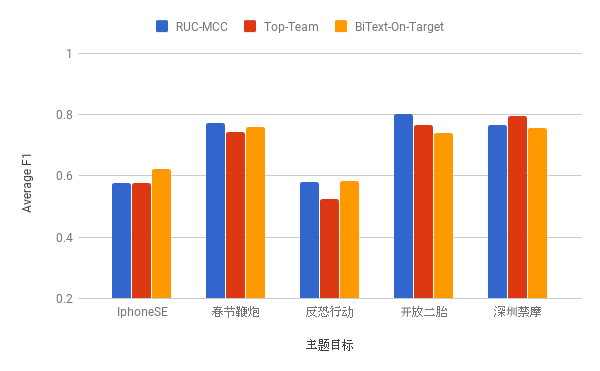
\includegraphics[width = 1.0\textwidth]{chart_nlpcc_best_model.png}
	\caption[rnn_vanish]{模型在SemeEval2016各主题目标平均F1值分布}
	\label{chart_nlpcc_best_model}
\end{figure}

本章节提出的BiText-On-Target模型在”春节放鞭炮“主题目标下取得了最好的0.75的平均F1值,RUC-MCC模型春节放鞭炮以外在其他主题模型上均有不错的性能,基于提取每个主题目标的关键字典的Top-Team在”深圳禁摩限电“主题目标上取得最好的0.794平均F1值。三个模型都有自己擅长的分析的主题目标,没有哪个模型能在所有主题目标中取得最好的指标。

上述模型在NLPCC数据集下的综合”支持“和”反对“的F1值和总体微平均F1值的性能如下表~\ref{nlpcc_res}~所示
\begin{table}[htbp]
	\caption[table123]{各模型在立场分析测试集中的性能表现(NLPCC 数据集)}
	\label{nlpcc_res}
	\vspace{0.5em}\centering\wuhao
	\begin{tabular}{cccccccc}
		\toprule[1.5pt]
		主题目标& $F_{favor}$&$F_{against}$&$F_{average}$ \\
		\midrule[1pt]
		RUC-MMC&0.6969&0.7243&0.7106\\
		Top-Team&0.6601&0.7186&0.6894\\
		BiText-On-Target&0.6761&0.7158&0.6984\\
		\bottomrule[1.5pt]
	\end{tabular}
\end{table}

本章提出的BiText-On-Target模型的性能可在NLPCC2016数据集上取得总微平均F1性能第二名,表明本章提出的BiText-On-Target模型是有效的,但是其性能和基于特征工程的RUC-MMC还有少了0.012差距,因此模型在立场分析建模上还有些许的不足,后续也可在此模型的基础上,更深入研究文本立场分析的问题。



\BiSection{本章小结}{}
本章介绍了基于条件编码LSTM模型的文本立场分析上的工作,受条件编码在文本蕴含任务上性能突破,将条件编码模型引入到文本立场分析任务。本章也简介了下SemEval2016和NLPCC2016两个社交媒体数据集,且说明评测的指标。对于立场分析中主题目标信息是否能促进文本立场分析的性能进行了探究,在两个数据集上设计了多组对比实验,实验证明以独立编码融合主题目标信息和文本信息的模型和直接单独编码文本信息的模型性能差距不大,而以条件编码融合主题目标信息和文本信息能提高文本立场分析的性能,得出以合适的方式引入主题目标信息对文本立场分析有促进作用,结合文本立场分析的特点,改进了条件编码模型,在两个数据集上的性能都优于原有模型,最好在中英文数据集上取得微平均F1值分别为0.698和0.671。通过对比两个数据集其他模型,条件编码LSTM模型均有不错的效果,表明本章提出的模型的有效性。




\begin{equation}\label{conv1} z_t=\alpha_g(W_zx_t+U_zh_{t-1}+b_z) \end{equation}
\begin{figure}[htbp]
	\centering
	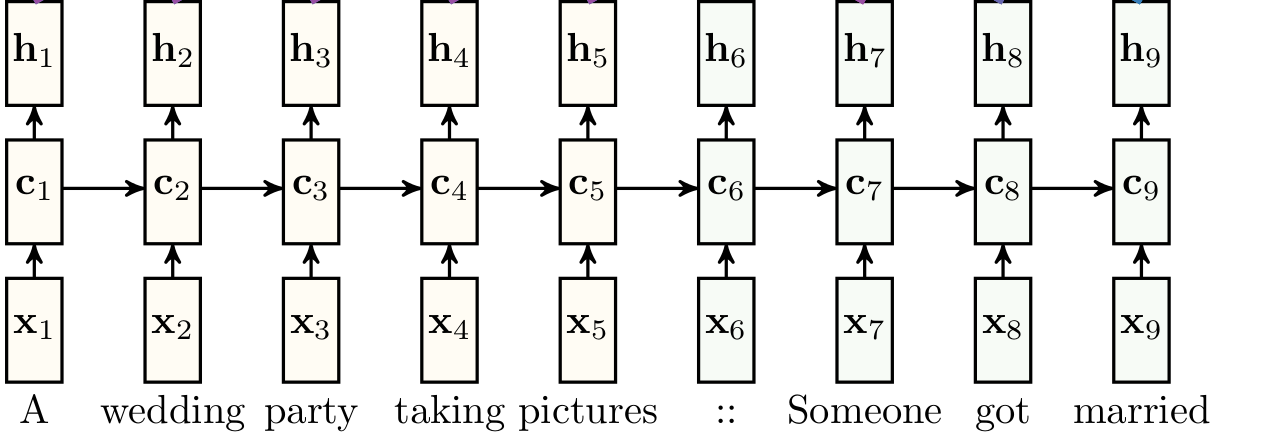
\includegraphics[width = 0.8\textwidth]{conditional_encoding.png}
	\caption[rnn_vanish]{条件编码长短期记忆}
	\label{hehehe}
\end{figure}

